\section{Variantendiskussion}
\label{sec:Variantendiskussion}
In der Entwurfsphase sollen aus den Anforderungen der Analysephase Modelle der zu entwickelten Software entstehen, die die konkreten Hardware- und Softwarebezogenen Anforderungen berücksichtigen. Diese Modelle gelten dann als unmittelbare Vorlage für die sich anschließende Implementationsphase. (vgl. \cite[S. 69]{dumke-2003})

Zu Beginn soll eine Marktrecherche durchgeführt werden, um bestehende Lösungen zu analysieren und auf Eignung zu Prüfen. Mit den gewonnen Erkenntnissen soll dann abgewägt werden ob Standartsoftware beschafft werden kann oder eine eigenentwicklung Veranlasst wird.
%Das erfolgt im Rahmen einer Variantendiskussion, in der verschiedene Ansätze und Technologien zur Umsetzung der Software bewertet werden.

Letztendlich soll der Programm- und Datenentwurf mithilfe geeigneter Modelle erarbeitet werden. Dies umfasst die Festlegung der Softwarearchitektur, der Datenstruktur sowie etwaiger Schnittstellen und der grafische Oberfläche.

\subsection{Marktrecherche}
\label{sec:Marktrecherche}
Im Rahmen der Marktanalyse wurden drei verschiedene Softwarelösungen für die Anwesenheitsplanung verglichen. Das Ziel dieser Analyse war es, Akquisitionsoptionen für das geplante Softwareprojekt zu ermitteln. Um Entscheidungen über die Eignung treffen zu können, wurden die Softwareprodukte auf den Erfüllungsgrad der Anforderungen geprüft. Dafür wurde eine Bewertungsmatrix erstellt, die funktionale- als auch nichtfunktionale Anforderungen beinhaltete. Dabei wurden die Kriterien so gewählt und gewichtet das zwingend erforderliche Anforderungen höher gewichtet wurden als optionale Anforderungen.

%TODO:Tabelle muss ordentlich Platziert werden
\begin{figure}[htb]
    \centering
    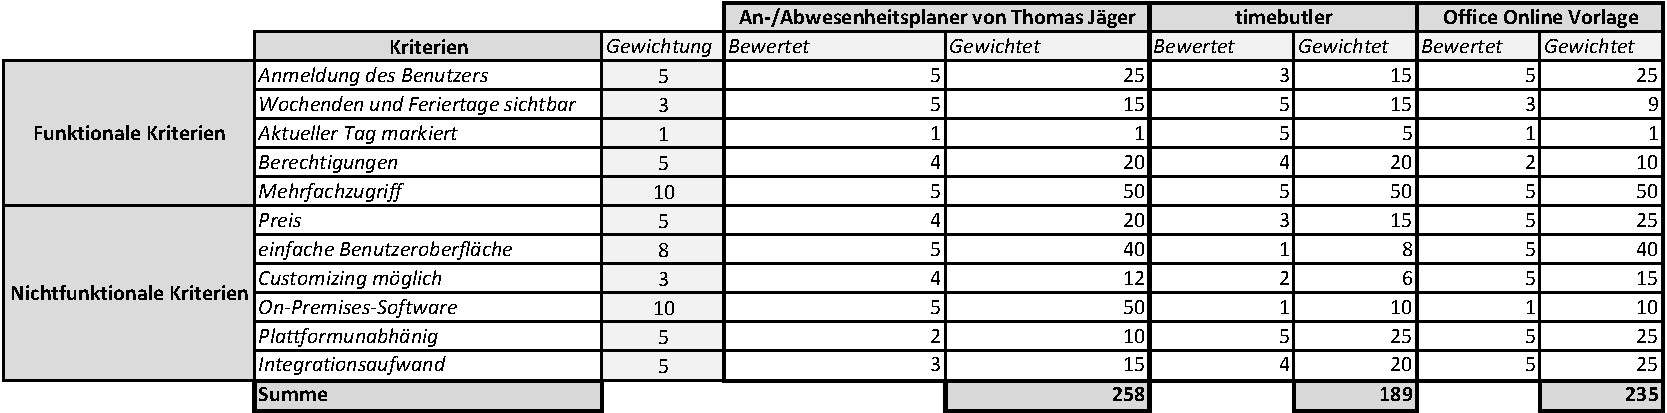
\includegraphics[width=0.9\textwidth,angle=0]{abb/Markterkundung.pdf}
    \caption[Beschreibung]{ Tabelle Markterkundung}
    \label{tab:Markterkundung}
\end{figure}

\subsubsection{An-/Abwesenheitsplaner von Thomas Jäger}
\label{sec:AnAbwesenheitsplaner}
Die erste betrachtete Software, der An-/Abwesenheitsplaner von Thomas Jäger, zeichnete sich durch die besonders intuitive Benutzeroberfläche aus. Bei der Betrachtung der anderen funktionalen Kriterien wurde festgestellt, dass die Software alle benötigten Anforderungen erfüllt und damit für den Einsatz geeignet ist. Negativ zu bewerten ist allerding, das die Software nur als Windows Programm zur Verfügung steht und damit nicht Plattformunabhängig eingesetzt werden kann. Zudem müsste ein solches Programm auf jedem Client PC im SMK installiert werden um die Software für alle Nutzbar zu machen. Damit ergibt sich ein hoher initialer Integrationsaufwand und auch späterer Wartungsaufwand den es zu berücksichtigen gilt. (vgl. \cite{AnAbwesenPlaner})


%Die Benutzerfreundlichkeit wurde jedoch als etwas komplex und steil eingestuft, was eine gewisse Einarbeitungszeit erforderte. Zudem war der Support nur eingeschränkt verfügbar und die Preisgestaltung vergleichsweise hoch. (vgl. \cite{AnAbwesenPlaner})
\subsubsection{timebutler}
\label{sec:timebutler}
Das zweite Programm namens timebutler überzeugte hingegen durch seine Plattformunabhängigkeit. Damit könnte es ohne großen Integrationsaufwand im SMK eingeführt und betrieben werden. Die Software bietet alle geforderten Funktionalitäten hat jedoch eine komplizierte Benutzeroberfläche und stellt viele Funktionen bereit die nicht benötigt werden. Das resultiert in höheren Anschaffungskosten als bei dem An-/Abwesenheitsplaner von Thomas Jäger. Besonders negativ ist zu bewerten, dass die Software zwar Plattformunabhängig ist, da sie auf Webtechnologien aufbaut, jedoch nicht als On-Premises-Software verfügbar ist. Damit müsste auf die Cloud des Anbieters zurückgegriffen werden was nicht gewünscht ist. (vgl. \cite{timebutler})

\subsubsection{Online Office Datei}
\label{sec:OnlineOffice}
Die dritte betrachtete Lösung ist die Verwendung einer Online Tabellenkalkulations Vorlage. Das würde es ermöglichen, die bereits vorhandenen Excel Tabellen für die Anwesenheitsplanung weiter zu verwenden. Durch das zurückgreifen auf Online Funktionalitäten die \zB von Microsoft mit Office356 oder mit Onlyoffice in Verbindung mit Nextcloud zur Verfügung stehen, kann man den gleichzeitigen Zugriff auf diese Listern erreichen. Damit würde man das Hauptproblem der einfachen Excel Dateien lösen. Doch auch hier müsste man im Falle des einsatzes von Office356 auf die Microsoft Cloud zurückgreifen. Desweiteren gibt es nur begrenzte Möglichkeit diese Excel Listen vor ungewollter Änderungen zu schützen und ein Berechtigungskonzept durchzusetzten.

\subsubsection{Auswertung der Marktrecherche}
\label{sec:AuswertungMarktrecherche}
Nach Betrachtung der drei Programme wurde festgestellt, dass keines der drei für eine Akquisition in frage kommt, da jedes seine individuellen Schwachstellen mit sich bringt. Der An-/Abwesenheitsplaner von Thomas Jäger wäre von allen die beste Option, da es eine benutzerfreundliche Oberfläche, eine solide Funktionalität und eine angemessene Preisgestaltung vereint. Die Plattformunabhängigkeit ist jedoch im SMK ein großer Faktor, da sich das neue Programm möglichst gut in die vorhandene Infrastruktur einfügen soll. Deswegen wurde sich gegen eine Akquisition von Standartsoftware entschieden. Um die geforderten Funktionalitäten abzubilden ohne dabei die Schwachstellen der Analysierten Programme inkauf nehmen zu müssen wurde ich für eine Eigenentwicklung der Software entschieden.

\subsection{Eigenentwicklung}
\label{sec:Eigenentwicklung}
Für die Umsetzung wurde Referat 12 mit der Entwicklung der Softwarelösung beauftragt. Die benötigten Hard- und Softwareressourcen vom SMK bereitgestellt und der zeitliche Rahmen für das Projekt wurde mit 32 Arbeitstagen angesetzt. Die genaue Aufschlüsselung des Projektablaufes siehe \ref{abb:Gantt}.

Für die Entwicklung der Software sethen dem Entwickler ein voll ausgestatteter Arbeitsplatz, sowie mehrere virtuelle Maschinen im Rechenzentrum zur Verfügung. Damit hat der Entwickler freie Hand bei der Umsetzung. Zu beachten ist jedoch, dass nach Möglichkeit auf die bestehende Infrastruktur zurückgegriffen bzw. berücksichtigt wird.


\subsection{Umsetzungsvarianten}
\label{sec:Umsetzungsvarianten}
Nach eingehender Analyse der Anforderungen und einer umfassenden Markterkundung wurden verschiedene Umsetzungsvarianten für das geplante Softwareprojekt des Anwesenheitsplaners untersucht. Dabei wurden insbesondere zwei Architekturansätze betrachtet: die monolithische Anwendung und die Client-Server-Architektur. Der Begriff der Architektur in der Softwareentwicklung ist dabei nur schwer zu definieren. In den folgenden Absätzen betrachte ich deswegen eine gemischte Form der System- und Software Architektur.

\subsubsection{monolithische Architektur}
\label{sec:monolithisch}
%TODO:was ist monolitisch
Die monolithische Architektur würde eine eigenständige Anwendung bedeuten, die auf den Client PCs installiert wird. Bei diesem Ansatz ist das Programm in der Lage, alle erforderlichen Komponenten und Dienste bereitzustellen. Dieser Ansatz ist vor allem dann geeignet, wenn die Anwendung auf einer spezifischen Plattform ausgeführt werden soll und keine Notwendigkeit für eine verteilte Architektur besteht. Da die monolithische Architektur sowohl das User-Interface als auch die Logik beinhaltet, entfällt der zusätzliche Bedarf an einem dedizierten Server für die Logik. Nachteil hierbei ist die eingeschränkte Flexibilität, da ein solches Programm an das System gebunden ist für das es Entwickelt wurde.

\subsubsection{Client-Server-Architektur}
\label{sec:ClientServer}
%TODO:Was ist Clien-Server
Die zweite betrachtete Option war die Client-Server-Architektur, die bei webbasierten Anwendungen mit einem Backend-Server und einer Datenbank zum Einsatz kommt. Bei dieser Architektur werden die Funktionen auf mehrere Schichten aufgeteilt. Der Backend-Server ist für die Verarbeitung der Anfragen und die Bereitstellung von Daten zuständig, während die Datenbank die persistente Speicherung der Daten ermöglicht. Der Benutzer interagiert mit dem System über das Frontend, das auf dem Client läuft. Um zu Kommunizieren sendet der Client Anfragen an den Server und erwartet entsprechende Antworten. Die Kommunikation zwischen Client und Server erfolgt dann über ein Netzwerkprotokoll wie HTTP. Ein Nachteil ist dabei die ständige Netzwerkabhängigkeit der Clients um den Dienst Nutzen zu können.

\subsubsection{Vergleich}
\label{sec:Vergleich}
Beide %TODO: der shit muss in ordnung gebracht werden!

Nach sorgfältiger Abwägung der Vor- und Nachteile beider Ansätze wurde beschlossen, auf eine Client-Server-Architektur mit Frontend und Backend zu setzen, und eine Webentwicklung anzustreben. Die Verwendung von Webtechnologien bringt den Vorteil der plattformunabhängigen Verfügbarkeit der Anwendung. Benutzer können von verschiedenen Geräten aus, die einen Webbrowser unterstützen, auf den Anwesenheitsplaner zugreifen. Darüber hinaus erleichtert die Verwendung von HTTP die Kommunikation zwischen Client und Server.

Insgesamt bietet die gewählte Client-Server-Architektur mit Frontend und Backend die besten Voraussetzungen für die Umsetzung des Anwesenheitsplaners. Durch die Webentwicklung wird eine flexible, plattformunabhängige Anwendung geschaffen, die sowohl die Benutzeranforderungen erfüllt als auch die Möglichkeit bietet, zukünftige Erweiterungen und Skalierungen problemlos umzusetzen.


\subsection{Programm und Datenentwurf}
\label{sec:ProgrammUDatenentwurf}